\section{Method}
\label{sec:method}

\begin{figure*}[t]
    \centering
    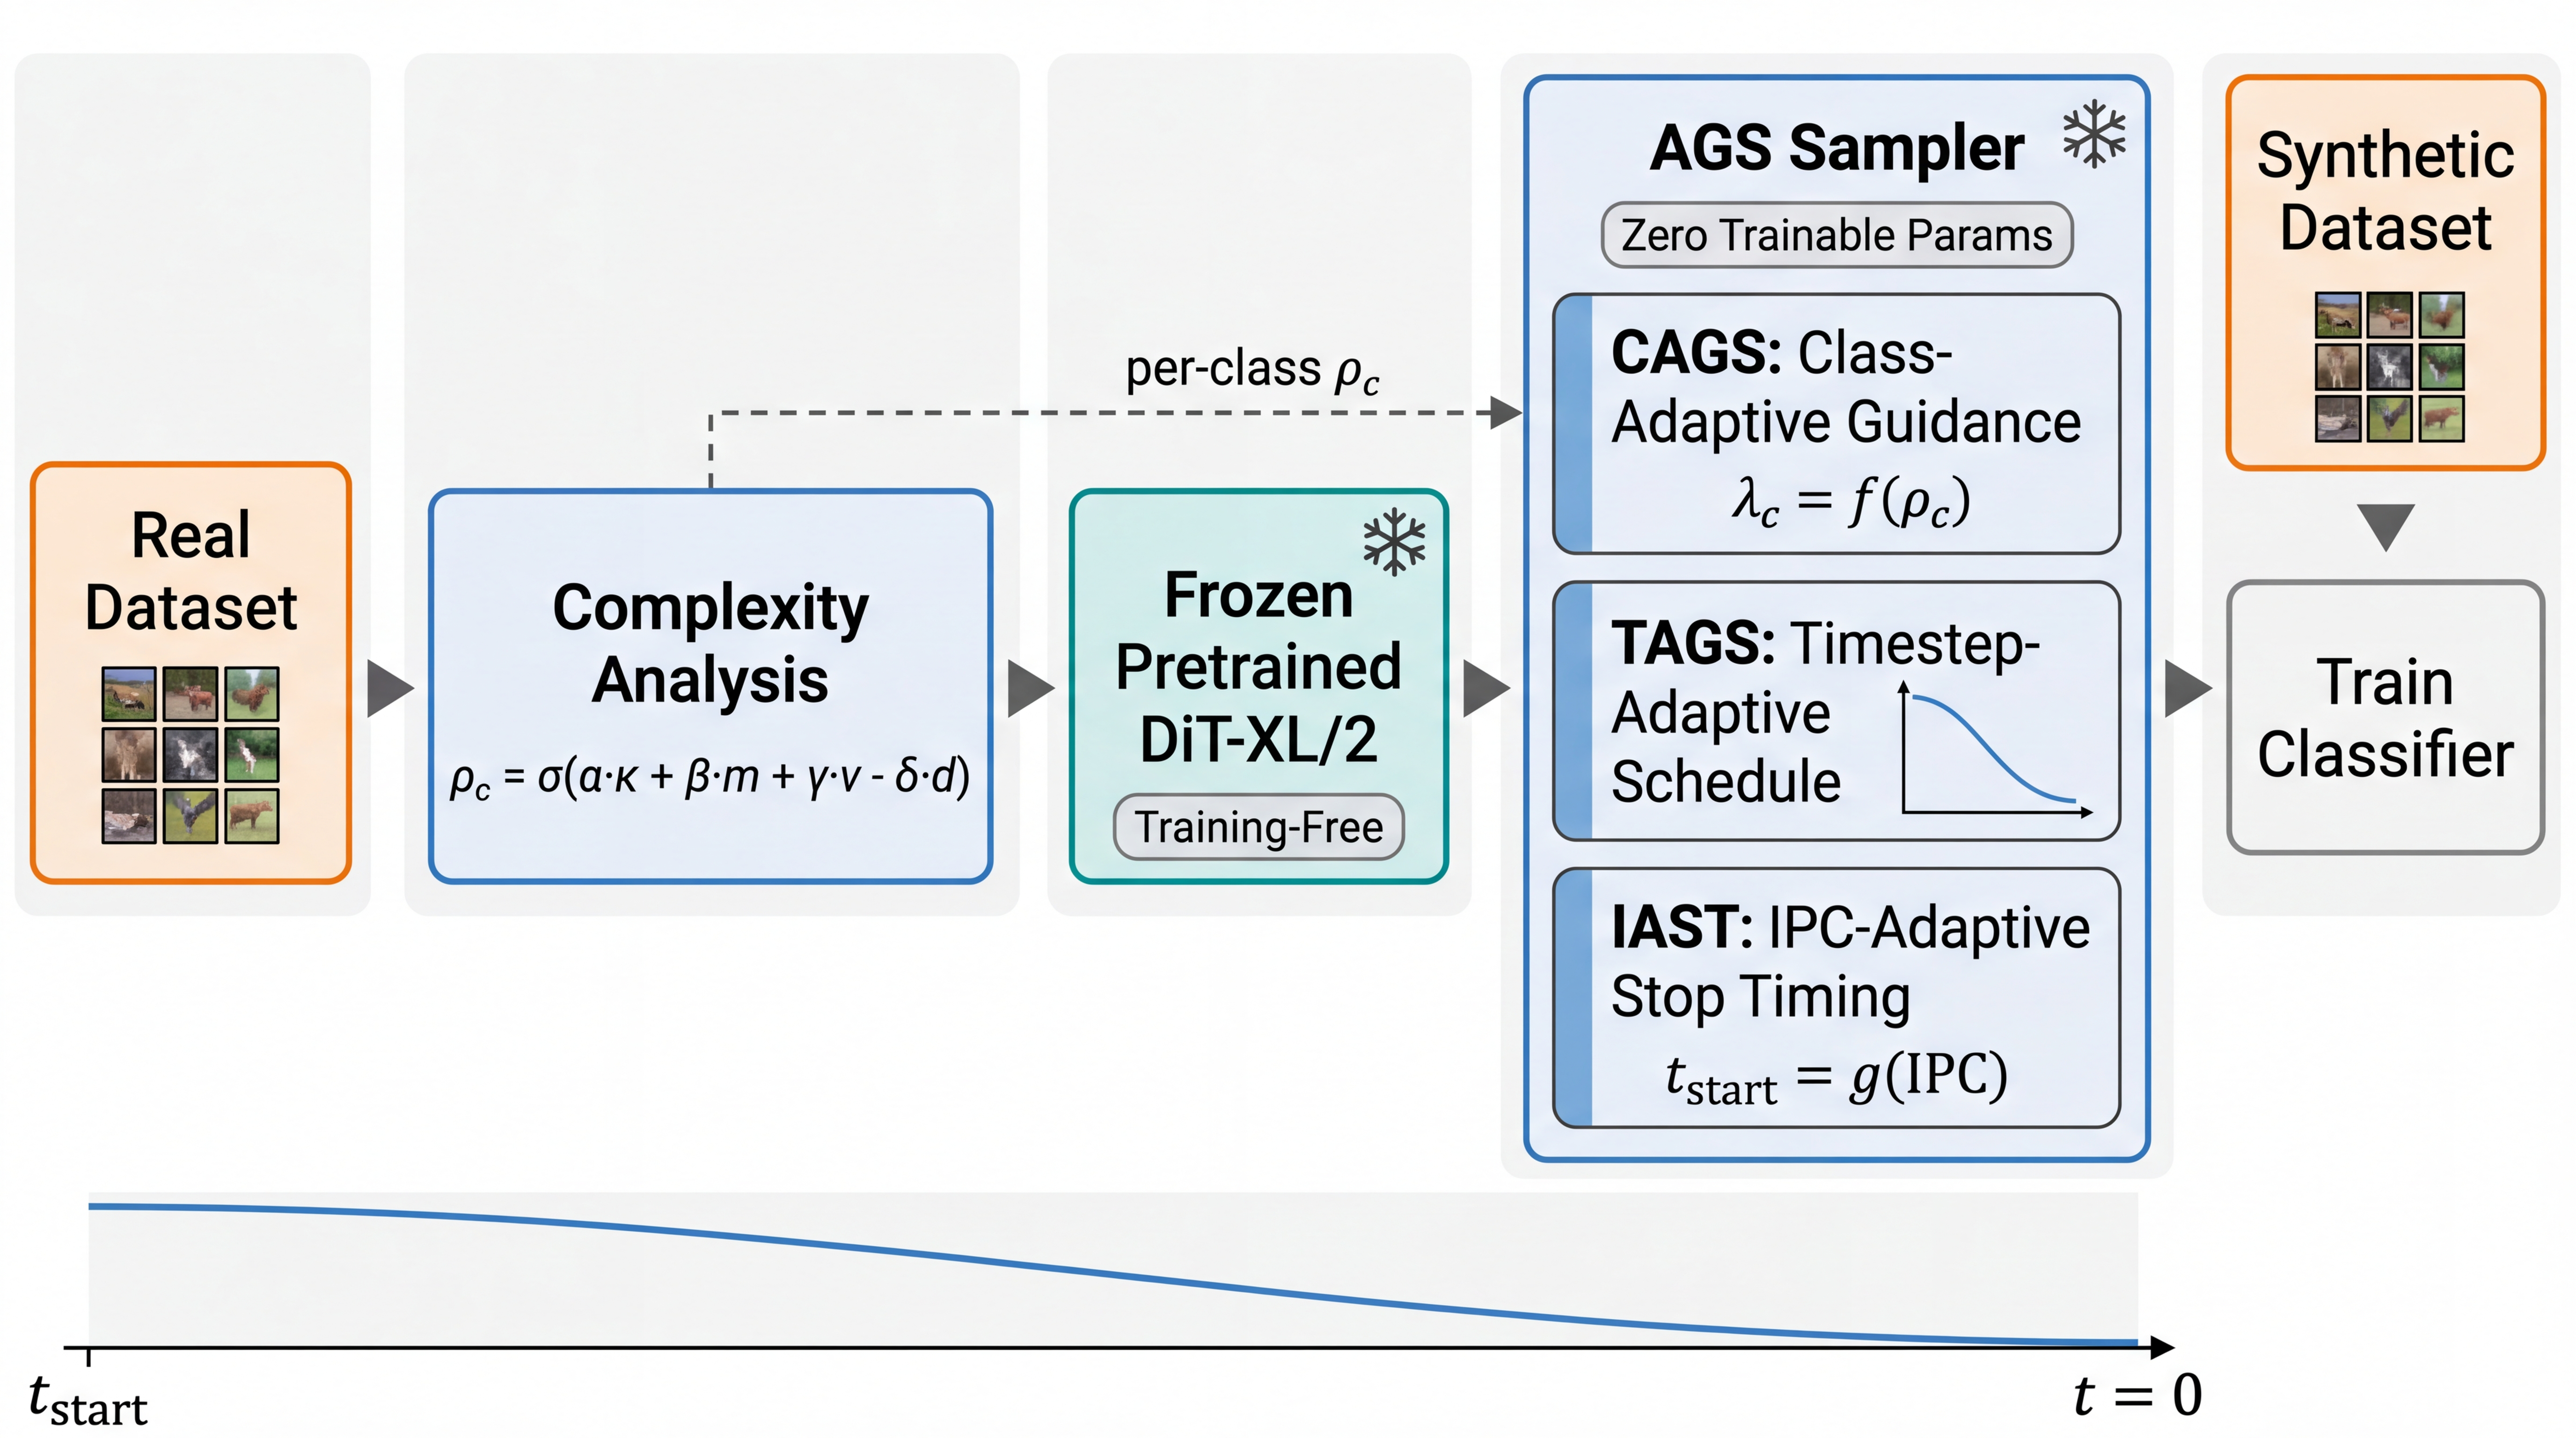
\includegraphics[width=\textwidth]{figures/framework.jpg}
    \caption{Overview of the \ags{} framework. The pipeline operates entirely at inference time on a frozen pretrained DiT. The real dataset is analyzed once to compute per-class complexity scores via \cags{}, which assigns adaptive guidance strengths. Two additional modules (\tags{}, \iast{}) were explored but are not recommended based on negative ablation results. No gradient computation or model training is required.}
    \label{fig:framework}
\end{figure*}

\ags{} enhances the training-free dataset distillation pipeline of MGD$^3$~\cite{chansantiago2025modeguided} by replacing its globally fixed classifier-free guidance with per-class adaptive guidance. \Cref{fig:framework} provides an overview of the framework. The core module, \cags{} (Section~\ref{sec:cags}), assigns a per-class guidance strength based on a multi-factor complexity metric. We additionally explored two complementary modules---\tags{} and \iast{} (Section~\ref{sec:tags-iast})---which address the temporal and IPC-budget axes respectively; both are investigated but ultimately not recommended based on negative ablation results.

\subsection{Background: Diffusion Models and Classifier-Free Guidance}
\label{sec:background}

Denoising diffusion probabilistic models (DDPMs)~\cite{ho2020denoising} learn to reverse a gradual noising process. Given a data sample $\mathbf{x}_0 \sim q(\mathbf{x}_0)$, the forward process corrupts it over $T$ timesteps according to a variance schedule $\{\beta_t\}_{t=1}^T$:
\begin{equation}
    q(\mathbf{x}_t \mid \mathbf{x}_0) = \mathcal{N}(\mathbf{x}_t; \sqrt{\bar{\alpha}_t}\,\mathbf{x}_0,\, (1 - \bar{\alpha}_t)\,\mathbf{I}),
    \label{eq:forward}
\end{equation}
where $\bar{\alpha}_t = \prod_{s=1}^t (1 - \beta_s)$. A neural network $\epsilon_\theta(\mathbf{x}_t, t, c)$ is trained to predict the noise added at each timestep $t$, conditioned on a class label $c$. The reverse process generates samples by iteratively denoising from $\mathbf{x}_T \sim \mathcal{N}(\mathbf{0}, \mathbf{I})$.

Classifier-free guidance (CFG)~\cite{ho2022classifierfree} enhances conditional generation by interpolating between the conditional and unconditional score predictions:
\begin{equation}
    \tilde{\epsilon}_\theta(\mathbf{x}_t, t, c) = (1 + \lambda)\,\epsilon_\theta(\mathbf{x}_t, t, c) - \lambda\,\epsilon_\theta(\mathbf{x}_t, t, \varnothing),
    \label{eq:cfg}
\end{equation}
where $\lambda \geq 0$ is the guidance scale and $\varnothing$ denotes the null (unconditional) class. The guidance scale $\lambda$ controls the quality--diversity trade-off: higher values produce samples that more faithfully adhere to the conditioning signal but sacrifice diversity, while lower values yield more diverse but potentially less class-accurate samples.

In MGD$^3$, the pretrained DiT-XL/2~\cite{peebles2022scalable} model is frozen, and synthetic images are generated by sampling from the reverse process using a fixed $\lambda$ for all classes and all timesteps. The generation begins from a high-noise timestep $t_{\text{start}}$ (rather than $T$), which controls the degree of structural diversity: starting from higher noise yields more varied samples, while starting from lower noise produces samples closer to the model's mode. We refer to the pair $(\lambda, t_{\text{start}})$ as the \emph{guidance configuration}.

\subsection{Class-Adaptive Guidance Strength (CAGS)}
\label{sec:cags}

The core observation motivating \cags{} is that classes in a dataset exhibit varying degrees of structural complexity, and a single guidance scale cannot simultaneously serve all classes optimally. A class with high intra-class variance (e.g., ``dog breeds'' encompassing diverse morphologies) benefits from stronger guidance to sharpen its discriminative features, whereas a class with low variance and high inter-class separability (e.g., ``parachute'' vs.\ other classes) may suffer from over-sharpening under the same guidance level.

\paragraph{Multi-factor complexity metric.}
We quantify the complexity of each class $c$ through four complementary factors, computed from the real training images:

\begin{enumerate}
    \item \textbf{Mode count} ($\kappa_c$): Captures the number of distinct visual modes within class $c$ via $K$-means clustering in the feature space. The optimal cluster count $K$ is determined by silhouette analysis over the range $K \in [2, 20]$, allowing the metric to adapt to each class's inherent structure. Classes with more modes are inherently more complex.

    \item \textbf{Cluster entropy} ($H_c$): Measures the balance of cluster sizes produced by $K$-means. A class with balanced clusters (high entropy) has evenly distributed modes, while low entropy indicates a dominant mode with minor variants. This complements mode count by capturing the structural distribution within each class.

    \item \textbf{Intra-class variance} ($v_c$): Measures the dispersion of images within class $c$. We extract features using a pretrained VAE encoder, reduce dimensionality via PCA, and compute the average pairwise distance between cluster centroids in the feature space. Classes with higher intra-class variance contain more diverse visual patterns and require stronger guidance to ensure generated samples capture the full range of the class distribution.

    \item \textbf{Inter-class separability} ($d_c$): Measures how well class $c$ is separated from other classes. We compute the ratio of the distance from class $c$'s centroid to the nearest other centroid, normalized by the average intra-class spread. Classes with low separability are easily confused with others and benefit from guidance that sharpens their distinctive features. Our factor ablation reveals that separability produces near-constant guidance across classes and is the least effective single factor (Section~\ref{sec:factor-ablation}).
\end{enumerate}

\paragraph{Complexity score and guidance mapping.}
The four factors are combined into a per-class complexity score $\rho_c \in [0, 1]$ via a weighted sum:
\begin{equation}
    \rho_c = \sigma\!\left(s \cdot \left(\alpha\,\hat{\kappa}_c + \beta\,\hat{H}_c + \gamma\,\hat{v}_c - \delta\,\hat{d}_c\right) - c_0\right),
    \label{eq:complexity}
\end{equation}
where $\hat{\kappa}_c$, $\hat{H}_c$, $\hat{v}_c$, and $\hat{d}_c$ are min-max normalized versions of mode count, cluster entropy, intra-class variance, and inter-class separability respectively, $\sigma(\cdot)$ is the sigmoid function, $s$ is the slope, $c_0$ is the center, and $(\alpha, \beta, \gamma, \delta)$ are weighting coefficients. We use $(\alpha, \beta, \gamma, \delta) = (0.3, 0.3, 0.2, 0.2)$ throughout. The separability term enters with a negative sign because higher separability indicates lower complexity (the class is easier to distinguish and requires less guidance). The complexity score is then mapped to a per-class guidance scale:
\begin{equation}
    \lambda_c = \lambda_{\min} + (\lambda_{\max} - \lambda_{\min}) \cdot \rho_c,
    \label{eq:cags_mapping}
\end{equation}
where $[\lambda_{\min}, \lambda_{\max}]$ is the guidance range. Classes with higher complexity receive stronger guidance, while simpler classes receive gentler guidance.

\paragraph{Theoretical motivation: why cluster entropy drives adaptive guidance.}
The factor ablation in Section~\ref{sec:factor-ablation} reveals that cluster entropy is the most effective single complexity factor, while inter-class separability is the least effective. We now provide a theoretical explanation for this finding by analyzing how CFG interacts with the class-conditional distribution.

Under CFG with scale $\lambda$, the effective conditional distribution becomes
\begin{equation}
    p_\lambda(\mathbf{x} \mid c) \propto p(\mathbf{x} \mid c)^{1+\lambda} \, p(\mathbf{x})^{-\lambda},
    \label{eq:cfg_dist}
\end{equation}
which raises the class-conditional density to the power $(1+\lambda)$ while down-weighting the marginal. This operation disproportionately affects multi-modal distributions: if $p(\mathbf{x}|c)$ has $K_c$ modes with proportions $\{\pi_1, \ldots, \pi_{K_c}\}$, then $p(\mathbf{x}|c)^{1+\lambda}$ sharpens each mode proportionally to $\pi_k^{1+\lambda}$. As $\lambda$ increases, smaller modes shrink faster than the dominant mode, eventually collapsing to a single mode. The rate of this collapse is governed by the entropy $H_c = -\sum_k \pi_k \log \pi_k$.

\begin{proposition}
\label{prop:entropy}
Let $p(\mathbf{x}|c)$ be a class-conditional distribution with $K_c$ modes of proportions $\{\pi_k\}$. Define the mode-survival probability under guidance scale $\lambda$ as $S_c(\lambda) = \sum_k \mathbb{1}[\pi_k^{1+\lambda} > \tau]$ for a threshold $\tau \in (0,1)$. Then the critical scale at which the $j$-th mode collapses, $\lambda_j^* = \frac{\log \tau - \log \pi_j}{\log \pi_j}$, satisfies $\frac{\partial \lambda_j^*}{\partial H_c} < 0$: classes with higher cluster entropy collapse at \emph{lower} guidance scales, making them more sensitive to the choice of $\lambda$.
\end{proposition}

\begin{proof}[Proof sketch]
For a mode with proportion $\pi_k$, the sharpened weight under scale $\lambda$ is $\pi_k^{1+\lambda}$. The mode survives (remains above threshold $\tau$) when $\pi_k^{1+\lambda} > \tau$, i.e., $\lambda < \frac{\log \tau - \log \pi_k}{\log \pi_k} = \frac{\log \tau}{\log \pi_k} - 1$. For balanced modes (high entropy), all $\pi_k \approx 1/K_c$, so the collapse threshold is similar across modes but occurs at a lower $\lambda$ because $\log(1/K_c) < 0$ is large in magnitude. For a dominant mode (low entropy, $\pi_1 \gg \pi_k$ for $k > 1$), the dominant mode survives to much higher $\lambda$, so mode collapse is less consequential: the class is effectively unimodal and sharpening is safe. Formally, $\lambda_j^*$ is monotonically decreasing in $\pi_j$, and higher entropy implies more modes with small $\pi_k$, hence lower average collapse thresholds.
\end{proof}

This proposition explains the empirical findings: high-entropy classes (balanced multi-modal distributions) are sensitive to $\lambda$---too much guidance collapses modes and reduces intra-class diversity, while too little fails to sharpen discriminative features. These classes benefit most from \emph{adaptive} guidance that assigns an appropriate (not necessarily maximal) $\lambda$. Low-entropy classes (dominant single mode) are robust to any reasonable $\lambda$ because sharpening a unimodal distribution does not cause mode collapse. Inter-class separability, by contrast, is a property of the \emph{marginal} distribution $p(\mathbf{x}) = \sum_c p(c)\,p(\mathbf{x}|c)$ and does not affect the intra-class modality structure that governs guidance sensitivity. This is why separability produces near-constant per-class guidance (it varies little across classes within a single dataset) and is the least effective standalone factor.

\paragraph{Cache-based computation.}
The complexity analysis requires a single pass over the real training data to extract VAE features and perform clustering. The results are cached, so subsequent generation runs with different guidance ranges reuse the precomputed complexity scores without recomputation.

\subsection{Additional Explorations: TAGS and IAST}
\label{sec:tags-iast}

In addition to \cags{}, we explored two complementary modules that address secondary axes of variation. Both are investigated but ultimately \emph{not recommended} based on negative ablation results (Section~\ref{sec:module-ablation}); we describe them here to delineate the boundary of the per-class adaptation approach.

\paragraph{Timestep-Adaptive Guidance Schedule (TAGS).}
\tags{} replaces the constant $\lambda$ in Eq.~\eqref{eq:cfg} with a time-varying schedule $\lambda(t)$, concentrating guidance at high-noise timesteps where it shapes global structure and relaxing it at low-noise timesteps to avoid over-sharpening. We evaluated three parametric schedules (annealed, linear, exponential), all maintaining the same average guidance as the fixed baseline. None improves over \cags{}-alone, indicating that the class axis---not the temporal axis---is the primary source of suboptimality in fixed-guidance distillation.

\paragraph{IPC-Adaptive Guidance Range (IAST).}
\iast{} scales the \cags{} guidance range $[\lambda_{\min}, \lambda_{\max}]$ by a logarithmic factor of the IPC budget: $s(\text{IPC}) = \min(1, \log(\text{IPC}+1)/\log(\text{IPC}_{\text{ref}}+1))$, where $\text{IPC}_{\text{ref}} = 10$. At IPC $\geq$ 10, $s = 1$ and \iast{} is transparent; at IPC=1, $s \approx 0.29$, compressing the range to prevent over-sharpening of single images. Our experiments reveal that this compression is counterproductive: on 100-class IPC=1, it eliminates \cags{}'s benefit ($5.87\%$ vs.\ \cags{}-alone $6.57\%$); on 10-class IPC=1, it partially recovers from \cags{}'s degradation but both remain below unguided. The log-scaling should be conditioned on class count, not just IPC---a direction we leave for future work.

\subsection{\ags{} Sampler}
\label{sec:unified}

The \cags{} module composes into a single sampling procedure, as summarized in Algorithm~\ref{alg:ags}. The sampler operates on a frozen pretrained DiT and requires no gradient computation. The optional \tags{} and \iast{} modules (Section~\ref{sec:tags-iast}) can be inserted at the marked steps but are not recommended based on our ablation results.

\begin{algorithm}[t]
\caption{\ags{} Sampling (CAGS core)}
\label{alg:ags}
\begin{algorithmic}[1]
\Require Frozen DiT $\epsilon_\theta$, class $c$, complexity cache $\{\rho_{c'}\}_{c'=1}^C$
\Ensure Synthetic image $\mathbf{x}_0$
\State $\lambda_c \gets \lambda_{\min} + (\lambda_{\max} - \lambda_{\min}) \cdot \rho_c$ \Comment{CAGS per-class guidance}
\State $\mathbf{x}_{t_{\text{start}}} \sim \mathcal{N}(\mathbf{0}, \mathbf{I})$
\For{$t = t_{\text{start}}, t_{\text{start}}-1, \ldots, 1$}
    \State \textcolor{gray}{// Optional: $\lambda_t \gets \textsc{TAGS}(\lambda_c, t)$ \Comment{TAGS (not recommended)}}
    \State $\tilde{\epsilon} \gets (1 + \lambda_c)\,\epsilon_\theta(\mathbf{x}_t, t, c) - \lambda_c\,\epsilon_\theta(\mathbf{x}_t, t, \varnothing)$
    \State $\mathbf{x}_{t-1} \gets \text{DenoiseStep}(\mathbf{x}_t, \tilde{\epsilon}, t)$
\EndFor
\State \Return $\mathbf{x}_0$
\end{algorithmic}
\end{algorithm}

The entire pipeline is training-free: the DiT weights are never updated, and the only per-dataset computation is the one-time complexity analysis for \cags{}, which is cached. This makes \ags{} as simple to deploy as \mgd{} while substantially improving the quality of the distilled dataset through principled per-class guidance adaptation.
